%
% Sam 15: Trying out with no ``effot per user'' section. 
 %DC 12: I like the idea of trying to put everything together to think about what it means/how these different notions of effort come together.  I don't know if it works, though -- everything looks really close to the # posts analysis for me, and chars per user just feels like another metric.
\section{Putting It Together on Effort}  %% DC 12: Former "User Effort" -- bad name since other stuff is also user effort.

 %DC 12: These graphs looks a lot like the ones for number of posts, and I dislike the "cohort tails" showing up again here.  
\begin{figure*}[!tb]
\centering
\begin{subfigure}{.49\textwidth}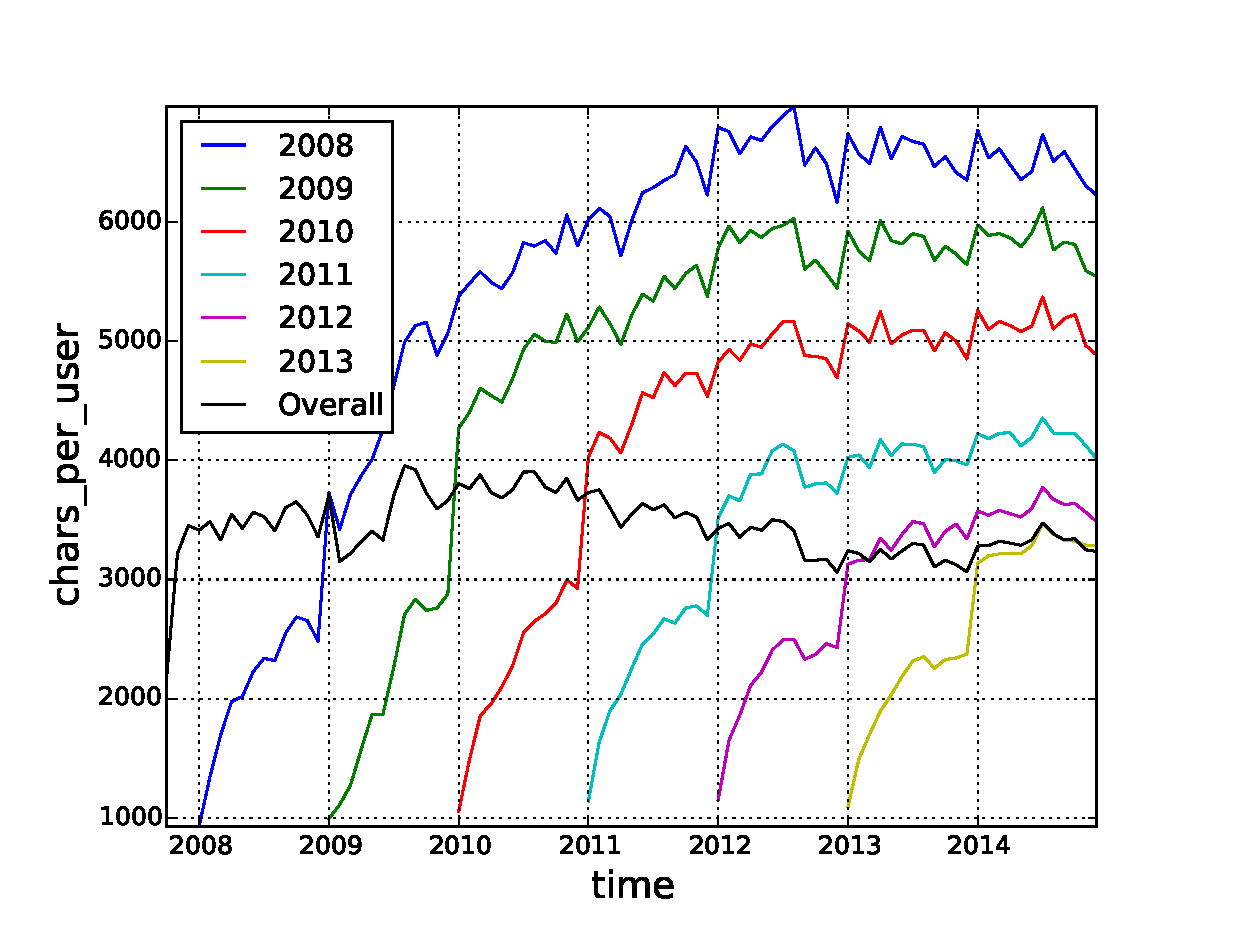
\includegraphics[scale=0.4]{./images/avr_comment_size_user_over_time_cohorts.eps}\caption{}\end{subfigure}
\begin{subfigure}{.49\textwidth}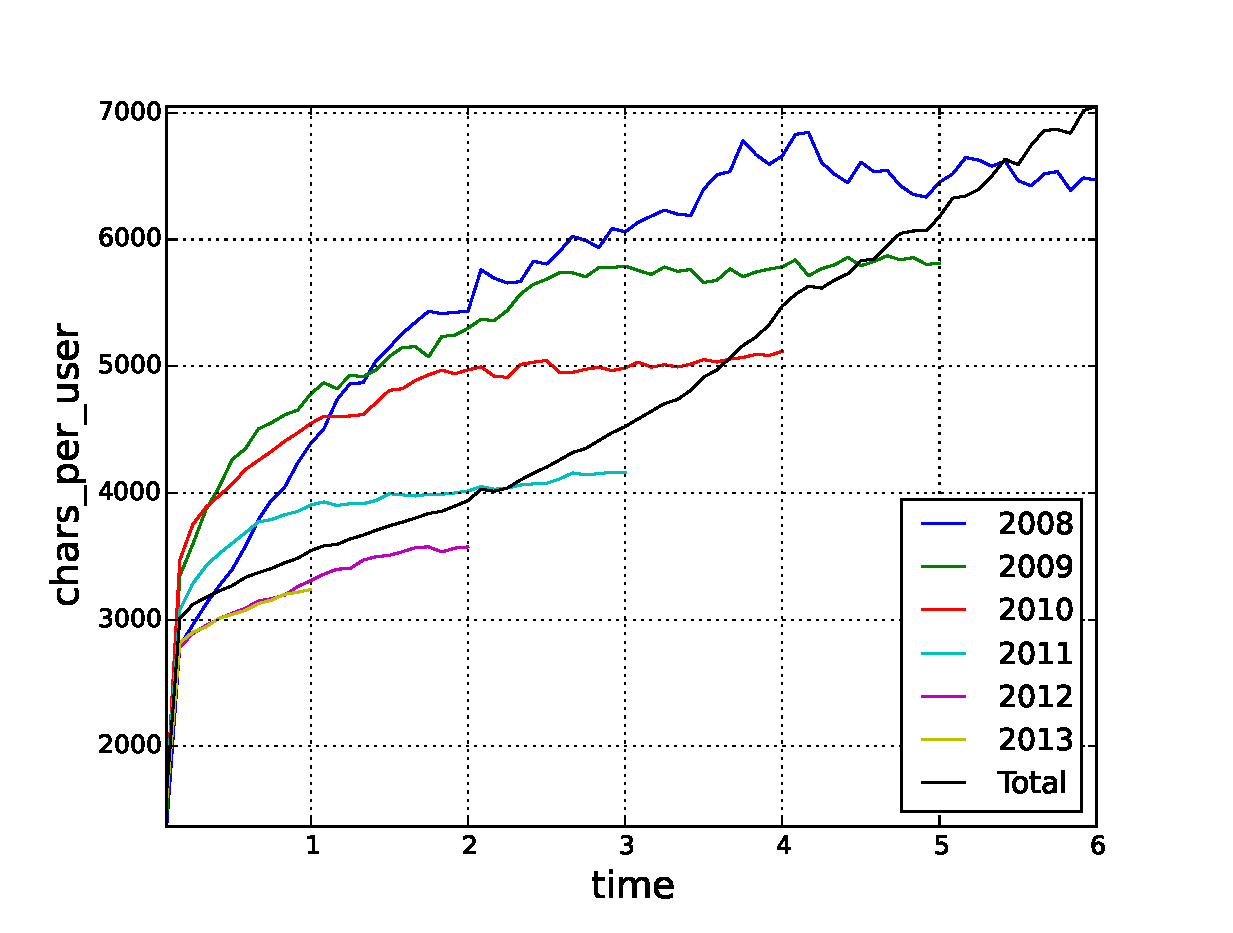
\includegraphics[scale=0.4]{./images/avr_comment_size_user_cohorts.eps}\caption{}\end{subfigure}
\begin{subfigure}{1\textwidth}
    %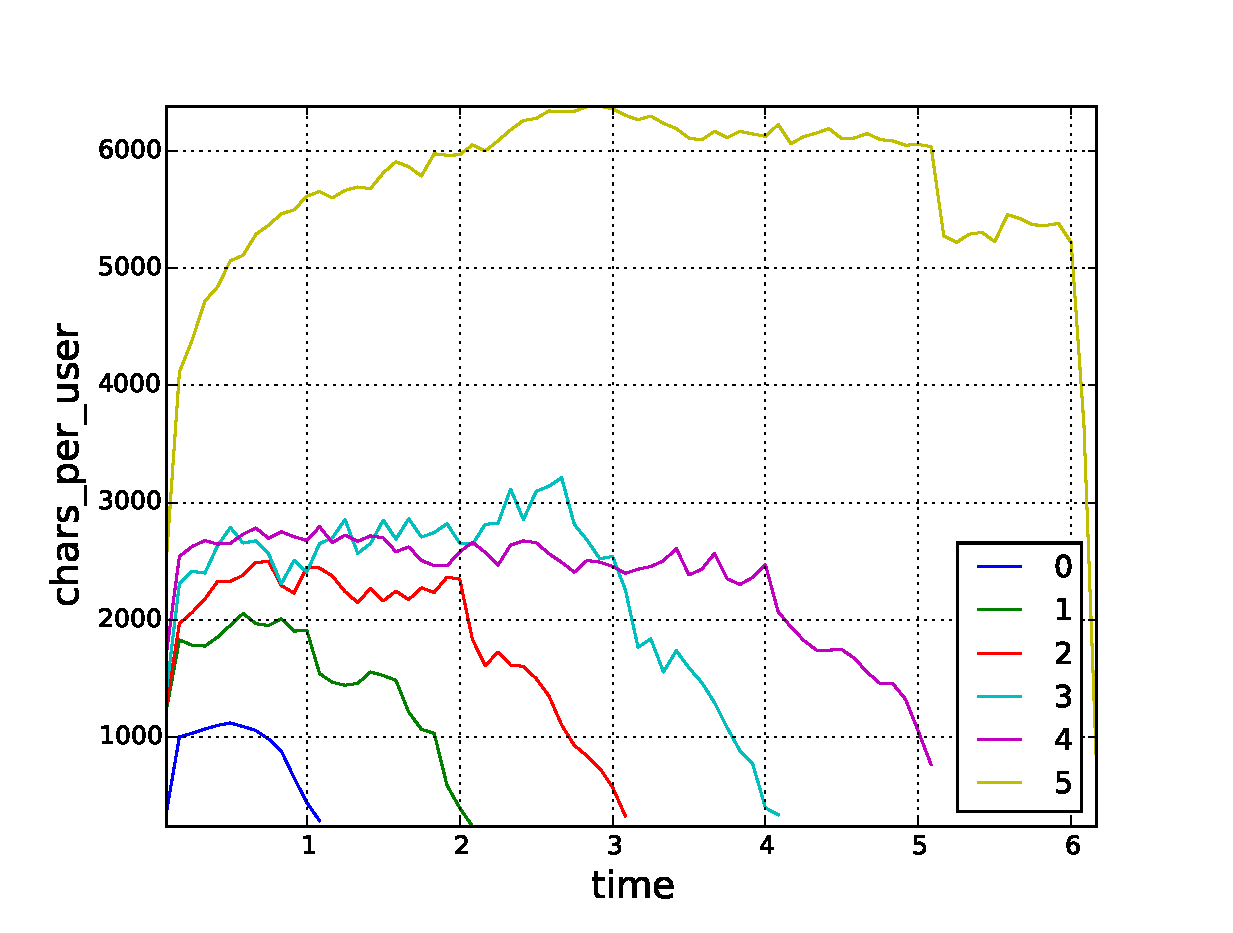
\includegraphics[scale=0.285]{./images/avr_comment_length_user_for_surviving_year_for_2009.eps}
    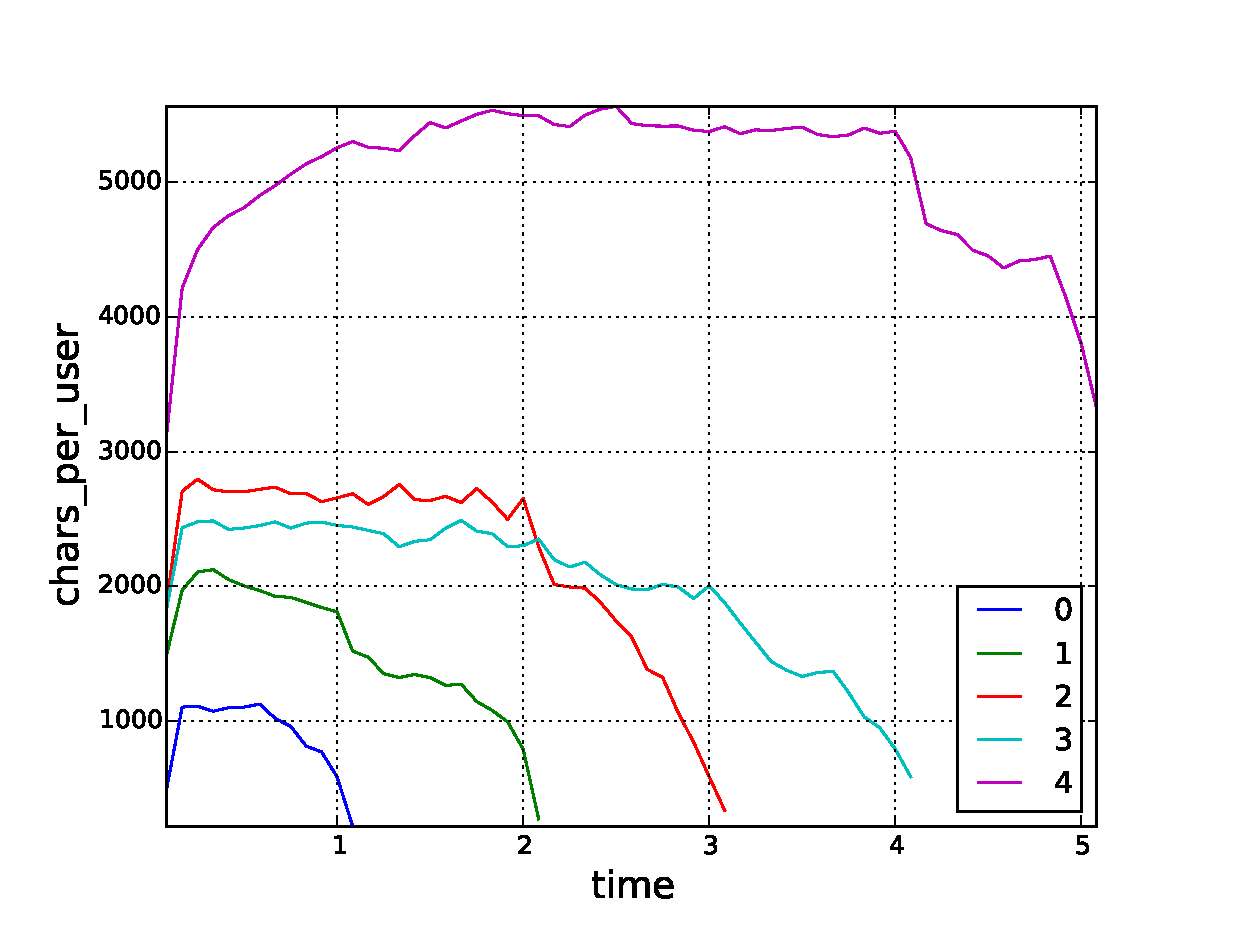
\includegraphics[scale=0.285]{./images/avr_comment_length_user_for_surviving_year_for_2010.eps}
    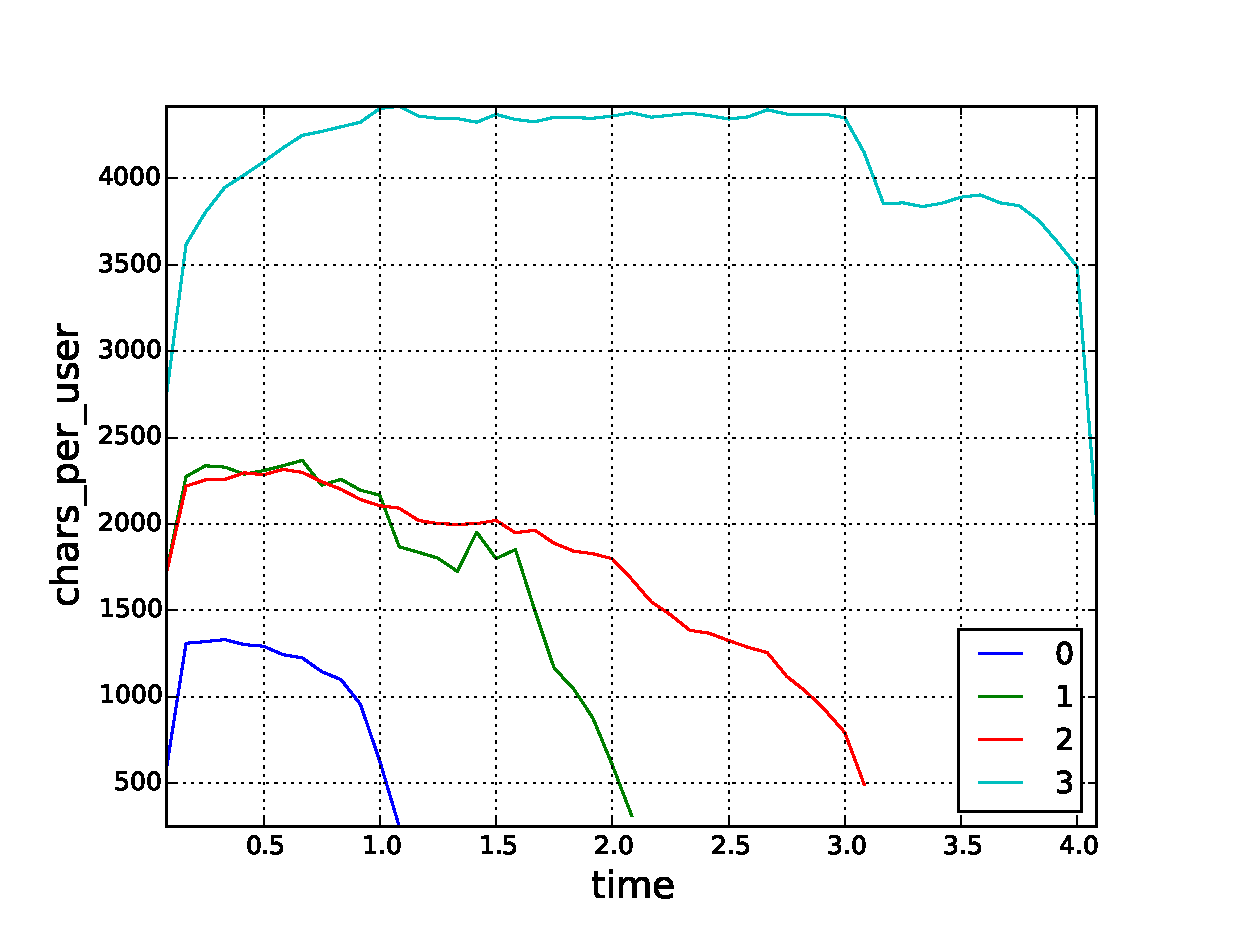
\includegraphics[scale=0.285]{./images/avr_comment_length_user_for_surviving_year_for_2011.eps}
    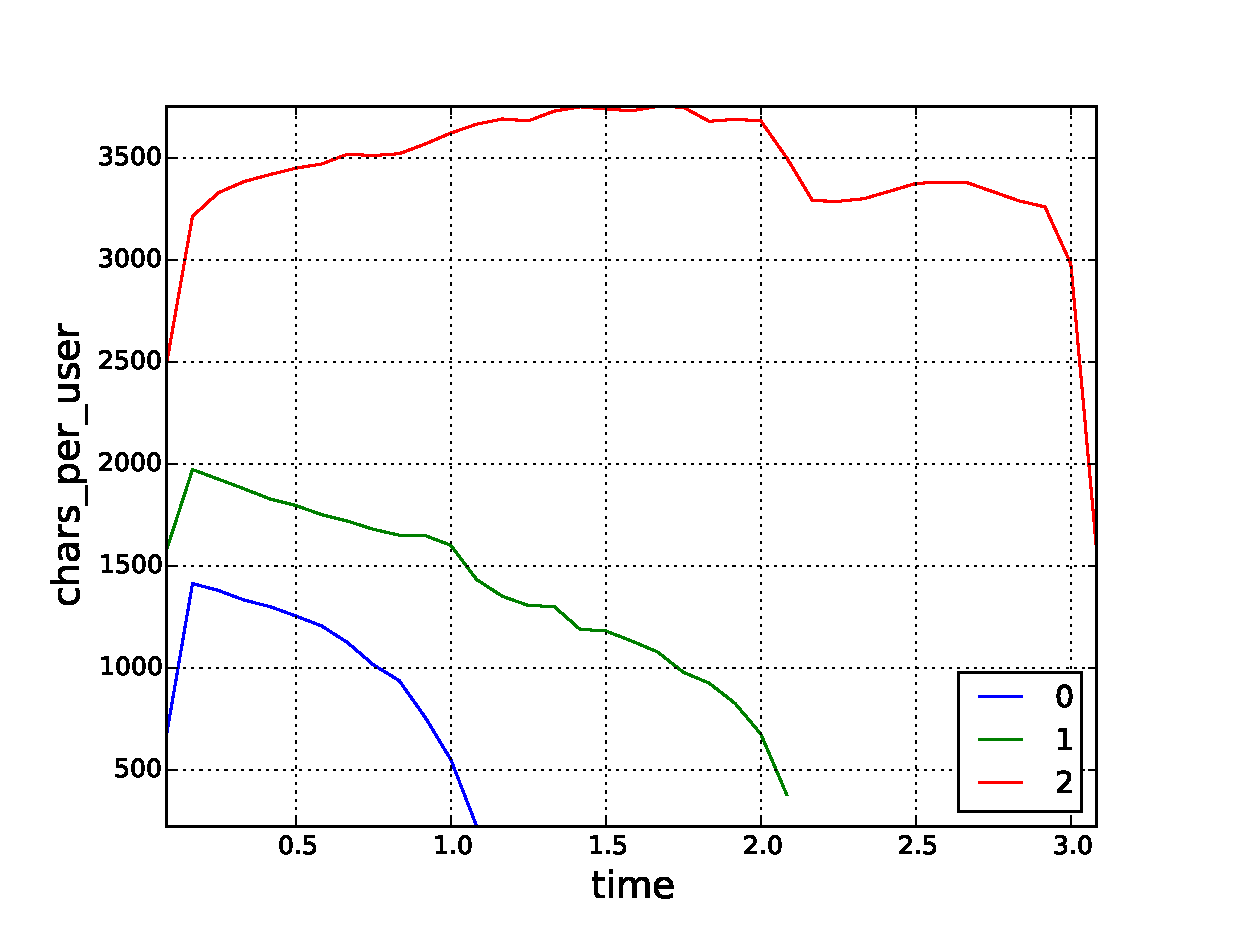
\includegraphics[scale=0.285]{./images/avr_comment_length_user_for_surviving_year_for_2012.eps}
\caption{}\end{subfigure}
\caption{Figure a shows the average number of written characters per user over clock time and Figure b from the user-referential time. Both figures show the cohorted trends and the overall users trends. Figure c, just as in Figure \ref{fig:avr_posts_per_user_for_surviving_year}, correspond to the cohorts of 2010, 11 and 12. They show the average number of written characters per user for users segmented by the number of years that the user survived in the network.}
\label{fig:chars_users}
\end{figure*}

In the previous sections we observed that the average effort per post for older cohorts increases as the users survive in the network. We also observed that users from older cohorts present higher effort per post for the same survived time than users from earlier cohorts. This means that as you age in reddit, you write more per post, and the earlier you joined, the more you write. But we also observed that users from earlier cohorts are commenting more per submission than users from older cohorts for the same time survived in the network. Could users be actually putting the same effort in terms of number of written characters, but younger users do it writing more, shorter comments while older users write less, longer comments? To investigate this, we follow the same steps as in the previous sections, analyzing the overall and cohorted behaviors, over time and from the user time referential.

In Figure \ref{fig:chars_users}a, we observe that during most of the time, the overall average number of characters written per user per month stays between 3000 and 3500, peaking near 2010 and showing a slightly downwards tendency throughout the end of 2014. The cohorted curves show a different growth pattern in comparison with the overall trend, mainly increasing and then leveling at different values, with older cohorts higher than younger ones. The decreasing overall trend happens because the latter cohorts have a much more significant weight in the average due to the increased number of users that joined reddit in the later years. This highlights the differences of the overall trend for the cohorted trend: while the overall shows a slightly decrease towards 2014, the cohorts show an increasing and leveling behavior. This can lead to wrong conclusions if not treated properly.

To further investigate how users evolve in the network, we see in Figure \ref{fig:chars_users}b the number of written characters per month per user from the user time referential for the overall average and the user creation date cohorted curves. We observe a sharp increase in the beginning of all lines due to the fact that a significant number of users only survive a very short time and the total amount of characters they contribute is considerably lower in comparison with the ones that survive for longer. The effect these users have in the analysis is concentrated in the leftmost part of the graphic, which improves the analysis in this referential. We can see that users, as they survive, write more characters per month. This can be due to the fact that users write more as they age and/or because users that write less die first and the surviving ones are the ones that write the most. From the user perspective, we see that the evolution of overall trend and the cohorted ones are significantly different. The overall trend shows a positive second derivative and apparently keep increasing for older users, while the cohorted ones have a negative one and eventually level. The conclusions about how users behave based on this can be quite misleading, specially considering that it is not reasonable for users to be forever increasing the amount of written characters as they survive.

To understand the increasing amount of written characters as the users age in the network, Figure \ref{fig:chars_users}c shows the per cohort set of figures that segments the users in each cohort according to the number of years survived. We can see clear trends of users leveling in different values of written characters per month according to the number of years they are likely to survive. This means that most of the increasing behavior of the user-time referential is due to users that write few characters dying earlier. Also, this suggests that the number of characters written per month by users conditioned on the cohort year is a good predictor of user survival.
